%%%%%%%%%%%%%%%%%%%%%%%%%%%%%%%%%%%%%%%%%
% Их сургуулийн оюутны тезис  
% LaTeX Загвар
% Version 2.3 (25/3/16)
%
% Энэ загвар нь дараах сайтаас авсан загварын монгол хувилбар юм.
% http://www.LaTeXTemplates.com
%
% Version 2.x major modifications by:
% Vel (vel@latextemplates.com)
%
% Анхдагч загварын эх үүсвэр:
% Steve Gunn (http://users.ecs.soton.ac.uk/srg/softwaretools/document/templates/)
% Sunil Patel (http://www.sunilpatel.co.uk/thesis-template/)
%
% Загварын лиценз:
% CC BY-NC-SA 3.0 (0)
%
%-----------------------------------------------------------------------
%	PACKAGES AND OTHER DOCUMENT CONFIGURATIONS
%-----------------------------------------------------------------------

\documentclass[
12pt, % Баримтын фонтын хэмжээ, сонголт: 10pt, 11pt, 12pt
oneside, % Хоёр талаар хэвлэж үдэхээр тохируулсан. Нэг тал бол комментыг арилга
%chapterinoneline,% Нэг мөрөнд бүлгийн дугаар, нэрийг гаргах
english, % babel багцын хэлний тохиргоо
onehalfspacing, % Мөр хоорондын зай. Сонголтууд: singlespacing, onehalfspacing, doublespacing
%draft, % Ноорог горимд шилжихийн тулд комментыг арилга(зураг, холбоос, hboxes гарахгүй)
nolistspacing, % Хэрэв мөр хоорондын зай onehalfspacing эсвэл doublespacing бол, жагсаалтын мөр хоорондын зайг single болгохын тулд комментыг арилга
%liststotoc, % Зураг/хүснэгт/бусад жагсаалтыг гарчигт оруулахын тулд комментыг арилга
%toctotoc, % Uncomment to add the main table of contents to the table of contents
%parskip, % Параграф хооронд зай оруулахын тулд комментыг арилга
%nohyperref, % hyperref багцыг ачаалахгүй бол комментыг арилга
headsepline, footsepline % Толгой мөрийн доогуур шугам татахын тулд комментыг арилга
]{MUST-Thesis} % Энэ класс файл нь баримтын бүтцийг тодорхойлно

\usepackage[utf8]{inputenc} % Олон улсын тэмдэгт оруулахад хэрэгтэй
\usepackage[T2A]{fontenc} % Олон улсын тэмдэгтийн гаралтын кодчилол
\usepackage[mongolian]{babel}
\usepackage{float}

\usepackage{titlesec}
\usepackage[table]{xcolor}
\usepackage{rotating} % эргүүлэх
\usepackage{enumitem}
\setlist{noitemsep}

\let\oldtabular\tabular
\let\endoldtabular\endtabular
\renewenvironment{tabular}
   {\bgroup\singlespacing\oldtabular}%
   {\endoldtabular\egroup}
\let\oldverse\verse
\let\endoldverse\endverse
\renewenvironment{verse}
   {\bgroup\singlespacing\oldverse}%
   {\endoldverse\egroup}

\usepackage{caption,longtable,ltcaption}
\DeclareCaptionJustification{nohyphen}{\hyphenpenalty=10000}
\captionsetup{justification=nohyphen}

\usepackage{pgf}
\usepackage{tikz} % зураг зурах
\usetikzlibrary{shapes,arrows,automata}

%-------------------------------------------------------------------------------
%	ӨНГӨНИЙ ШИНЭЧИЛСЭН ТОХИРГОО (Cream Brown & White Theme)
%-------------------------------------------------------------------------------
\definecolor{CreamBrown}{cmyk}{0.10, 0.25, 0.35, 0.15}    % Зөөлөн крем бор
\definecolor{SoftCream}{cmyk}{0.04, 0.10, 0.18, 0.02}     % Маш цайвар крем
\definecolor{PureWhite}{rgb}{1.0, 1.0, 1.0}               % Цэвэр цагаан
\definecolor{DarkCreamBrown}{cmyk}{0.15, 0.35, 0.45, 0.25} % Гүн бор (текст/код тодотгох)

\definecolor{Cover}{RGB}{255, 255, 255}                  % Нүүрний фон - Цагаан
\definecolor{Chapter}{cmyk}{0.10, 0.25, 0.35, 0.15}       % Бүлгийн фон - Крем бор

\definecolor{lightlightgray}{cmyk}{0.02, 0.04, 0.06, 0.00} % Кодны арын дэвсгэр - Маш цайвар крем
\definecolor{OliveGreen}{cmyk}{0.15, 0.35, 0.45, 0.25}     % Кодын түлхүүр үгс - Бор
\definecolor{CadetBlue}{cmyk}{0.10, 0.20, 0.30, 0.10}      % Кодын тайлбар - Зөөлөн бор туяа

\usepackage{listings}
\renewcommand{\lstlistingname}{Эх код} % Програмын эх код хэвлэх
\lstset{
language=C,                             % Code language
basicstyle=\linespread{1.0}\ttfamily,   % Code font
keywordstyle=\color{OliveGreen},        % Keywords font
commentstyle=\color{CadetBlue},         % Comments font
numbers=left,                           % Line nums position
numberstyle=\tiny,                      % Line-numbers fonts
stepnumber=1,                           % Step between two line-numbers
numbersep=5pt,                          % How far are line-numbers from code
backgroundcolor=\color{lightlightgray}, % Background color
frame=none,                             % A frame around the code
tabsize=2,                              % Default tab size
captionpos=t,                           % Caption-position
breaklines=true,                        % Automatic line breaking?
breakatwhitespace=false,                % Automatic breaks only at whitespace?
showspaces=false,                       % Dont make spaces visible
showtabs=false,                         % Dont make tabs visible
columns=flexible,                       % Column format
morekeywords={__global__, __device__},  % CUDA specific keywords
}

\usepackage[autostyle=false]{csquotes} % Ном зүйд хэлнээс хамаарсан хашилт оруулахад хэрэгтэй
\usepackage[backend=bibtex,natbib=true,sorting=none,sortcites]{biblatex} % Ном зүйд bibtex -г ашиглах

\addbibresource{references.bib} % Ном зүйн файл

\newcommand{\authorshipname}{Зохиогч эрхийн хамгаалал}
\newcommand{\abbrevname}{Товчилсон үгс}
\newcommand{\constantsname}{Физик тогтмолууд}
\newcommand{\symbolsname}{Таних тэмдэгтүүд}
\newcommand{\acknowledgementname}{Талархал}
\newcommand{\abstractname}{Хураангуй}
 
%-------------------------------------------------------------------------------
%	THESIS INFORMATION
%-------------------------------------------------------------------------------

\thesistitle{ «Милая» бэйкиригийн барааны нөөц бүртгэх систем }
\thesistype{Бие даалтын ажил}
\supervisor{Доктор (Ph.D, дэд профессор), Б. Долгорсүрэн}
\advisor{........................./Магистр Т. Золбоо/ }

\degree{Системийн шинжилгээ ба зохиомж}
\authorshort{2-р баг}
\authorlong{2-р баг}
\addresses{battogtoh.batushka@gmail.com}
\subject{Мэдээллийн технологи}
\keywords{\LaTeX{}, Тезис}
\university{\href{http://www.must.edu.mn}{Шинжлэх Ухаан Технологийн Их Сургууль}}
\department{Мэдээллийн технологийн салбар}
\deptchair{Дэд проф. PhD. А.Алтангэрэл}
\group{Судалгааны баг}
\faculty{\href{http://www.sict.edu.mn}{Мэдээлэл, Холбооны Технологийн Сургууль}}

\hypersetup{pdftitle=\ttitle}
\hypersetup{pdfauthor=\shortname}
\hypersetup{pdfkeywords=\keywordnames}
\hypersetup{allcolors=black}

\usepackage{longtable}
\begin{document}

\frontmatter % Агуулгын өмнөх хуудас дугаарлалт: i, ii, iii, iv... г.м.

\pagestyle{plain} % Тезисийн загварыг дуудах хүртэлх толгой мөрийн суурь загвар


%-------------------------------------------------------------------------------
%	TITLE PAGE
%-------------------------------------------------------------------------------
\pagecolor{Cover}
\begin{titlepage}
	\begin{center}
		
		{\scshape\LARGE \univname\par} % Их сургуулийн нэр
		{\scshape\Large \facname\par}\vspace{0.5cm} % Их сургуулийн нэр
		
		\begin{figure}[!htbp]
			\centering
			
\includegraphics[scale=0.2]{Figures/MUST_logo.png}
		\end{figure}
		
		\vspace{1cm}
		\hfill \large{\longname} \\
		
		\vspace{1cm}
		
		{\huge \bfseries \ttitle\par}\vspace{0.4cm} % Тезисийн нэр
		
		\vspace{3cm}
		\textsc{\Large {\thesisname}}\\ % Тезисийн төрөл
		
		\vfill
		
		\large {Улаанбаатар хот} \\
		{\large 2026 он}\\ % Date
		
	\end{center}
\end{titlepage}
\pagecolor{white}

%-------------------------------------------------------------------------------
%	SUBTITLE PAGE
%-------------------------------------------------------------------------------

\begin{titlepage}
    \begin{center}
        {\scshape\LARGE \univname\par} % Их сургуулийн нэр
        {\scshape\Large \facname\par}\vspace{0.5cm} % Факультет
        
        \vspace{2cm}
        \hfill \large{\deptname} \\
        
        \vspace{2cm}
        {\huge \bfseries \ttitle\par}\vspace{0.4cm} % Тезисийн нэр
        
        \vspace{2cm}
        
        \begin{flushleft} 
            \normalsize
            Хөтөлбөрийн индекс: \degreeid \\
            Хөтөлбөр: \degreename \\[1.5cm]
            \makebox[8cm][l]{\emph{Удирдагч:} \dotfill \supname} \\
            \vspace{0.4cm}
            \makebox[8cm][l]{\textit{Гишүүн:} \dotfill B241940031 Б.Баттогтох} \\
            \vspace{0.4cm}
            \makebox[8cm][l]{\textit{Гишүүн:} \dotfill В241940001 А.Гэрэл} \\
            \vspace{0.4cm}
            \makebox[8cm][l]{\textit{Гишүүн:} \dotfill В241940010 О.Батцэцэг} \\
            \vspace{0.4cm}
            \makebox[8cm][l]{\textit{Гишүүн:} \dotfill В241940022 Б.Мөнхзаяа} \\
            \makebox[8cm][l]{\textit{Гишүүн:} \dotfill В241940016 О.Ганзаяа} \\
        \end{flushleft}
        
        \vfill
        
        \large {Улаанбаатар хот} \\
        {\large 2026 он}\\
    \end{center}
\end{titlepage}
 % Нүүр хуудас
%-------------------------------------------------------------------------------
%	WORK PLAN & REVIEW PAGE
%-------------------------------------------------------------------------------

\begin{titlepage}

\vspace*{0.5cm}
Батлав. Удирдагч: 
\begin{flushright}
\makebox[4cm]{\dotfill} /\supname/
\end{flushright}

\begin{center}

\vspace*{2cm}
\textbf{{\large БИЕ ДААЛТЫН АЖЛЫН \\ ТӨЛӨВЛӨГӨӨ}}\\[0.5cm]

\textsc{\large Сэдэв: ''\ttitle''}\\[0.5cm]

\begin{tabular}{|c|p{7cm}|c|c|}
	%\rowcolor{gray!40}
	\hline
	№ & \makebox[7cm][c]{Ажлын бүлэг, хэсгийн нэр} & Бүлгийн дугаар & Дуусах хугацаа \\ \hline
	1 & {Бие даалт 1}         &  1, 2 & 2026-?-? \\ \hline
	2 & {Бие даалт 2}     & 3 & 2026-?-? \\ \hline
	3 & {Эцсийн хамгаалалт} & 1-3 & 2026-?-? \\ \hline
\end{tabular}

\vspace{2cm}
Төлөвлөгөөг боловсруулсан баг: \makebox[3cm]{\dotfill} /\shortname/

\end{center}

 % Төлөвлөгөө, гүйцэтгэл, шүүмжийн хуудас
%-------------------------------------------------------------------------------
%	DECLARATION PAGE
%-------------------------------------------------------------------------------
\begin{declaration}
\addchaptertocentry{\authorshipname}

\noindent \qquad Миний бие Б.Баттогтох  нь, ''{\ttitle}'' сэдэвт энэ ажил нь манай багийнх бөгөөд дараахыг нотолж байна. Үүнд:

\begin{itemize} 
\item Манай баг энэ ажлыг F.ITM311 хичээлийн хүрээнд бүхэлд нь буюу голлон хийсэн болно.
\item Бусад хүмүүсийн хэвлүүлсэн ажлаас зөвлөгөө авсан бол түүнийгээ үндэслэсэн болно.
\item Бусад хүмүүсийн ажлаас ишлэл хийхдээ гол эх үүсвэрийг нь заасан болно.
\item Манай багийн ажилд тусалсан голлох бүх эх үүсвэрт талархаж байна.
\item Ажлыг бусадтай хамтарсан бол алийг нь бусад хүмүүс хийсэн болохыг тодорхой заасан болно.
\end{itemize}
\bigskip
 
\noindent Гарын үсэг: \rule[-0.5em]{12.7em}{0.5pt}
\bigskip

\noindent Огноо: \rule[-0.5em]{15em}{0.5pt}

\end{declaration}

\clearpage

 % Мэдэгдлийн хуудас
\include{FrontBackMatter/Quotation} % Ишлэл хуудас
%-------------------------------------------------------------------------------
%	ABSTRACT PAGE
%-------------------------------------------------------------------------------

\addchaptertocentry{Хураангуй} % Хураангуйг гарчигт нэмэх

\begin{center}
{\scshape\Large \univname\par} % Их сургуулийн нэр
{\scshape\large \facname\par}\vspace{0.5cm} % Их сургуулийн нэр
{\huge\textbf{{Хураангуй}} \par}
\bigskip
{\Large{\ttitle} \par} % Тезисийн нэр
\bigskip

{\normalsize \shortname \par} % Зохиогчийн нэр
\addressname
\end{center}

% \textit{\textbf{Түлхүүр үгс: \keywordnames}}
\qquad
Уг систем нь салбар бүр дэх барааны нэр төрөл, үлдэгдэл ширхэгийг вэб дээр бодит цагийн горимоор харуулна. Хугацаа дуусах дөхсөн бүтээгтэхүүн тухайн өдрийн дэлгүүр хаахаас 3–4 цагийн өмнө автоматаар 30\%-ийн хямдралтай цэс рүү шилжих юм. Тооллого, борлуулалт, хямдралыг ингэж автоматаар холбосноор хүний ажиллагаанаас үүсэх алдааг бүрэн арилгана. Мөн хадгалах хугацаа болон хямдрах цагийг барааны ангилал бүрээр уян хатан тохируулах боломжтой тул хаягдлыг эрс багасгах давуу талтай. Энэхүү нэгдсэн тайлан мэдээлэл нь удирдлагад түргэн шуурхай, оновчтой шийдвэр гаргах боломжийг олгож байна. % Ажлын хураангуй
%-------------------------------------------------------------------------------
%	ACKNOWLEDGEMENTS
%-------------------------------------------------------------------------------

\begin{acknowledgements}
\addchaptertocentry{\acknowledgementname}

Энэхүү бие даалтын ажлыг хийж гүйцэтгэхэд туслалцаа үзүүлж, их зүйлийг зааж, чиглүүлж өгсөн удирдагч багш Доктор (Ph.D) Б.Долгорсүрэн, зөвлөх багш нартаа баярлалаа. \ldots

\end{acknowledgements}

 % Талархлын хуудас

%-------------------------------------------------------------------------------
%	LIST OF CONTENTS/FIGURES/TABLES PAGES
%-------------------------------------------------------------------------------

\tableofcontents % Гарчиг хэвлэх
\listoffigures % Зургийн жагсаалт хэвлэх
\listoftables % Хүснэгтийн жагсаалт хэвлэх

%-------------------------------------------------------------------------------
%	THESIS CONTENT - CHAPTERS
%-------------------------------------------------------------------------------

\mainmatter % Хуудасны тоон (1,2,3...) дугаарлалт эхлэнэ
\include{FrontBackMatter/udirtgal} % Ажлыг хэнд зориулсан
\pagestyle{thesis} % Хуудасны толгойг "thesis" загвар руу буцаах
\myformat % Бүлгийн нэрийг тусгай хуудсанд хэвлэх

\include{Chapters/udirtgal}
% Бүлэг 1

\chapter{Судалгааны хэсэг} % Бүлгийн нэр
\label{Chapter1} % Энэ бүлэг рүү ишлэл хийх бол \ref{Chapter1} командыг ашигла 

%-------------------------------------------------------------------------------
\section*{Системийн зорилго}

Жижиг, дунд үйлдвэрлэлийн газар (бэйкири)-ын өдөр тутмын үйл ажиллагаанд шаардлагатай барааны нөөцийн тооллого, борлуулалттай уялдсан автомат хасалт, бүтээгдэхүүний ангилал бүрийн хадгалах хугацаа (Shelf Life)-д суурилсан автомат хямдралын жагсаалт үүсгэх процессуудыг хамарсан мэдээллийн системийн зохион байгуулалт, шаардлагыг судлах, дүн шинжилгээ хийхэд чиглэгдэнэ. 

%-------------------------------------------------------------------------------
\section{Сэдэв сонгох}
Тайлангийн сэдэв: «Милая» бэйкириний барааны нөөц бүртгэх систем.

%-------------------------------------------------------------------------------
\section{Системийн зорилт}
\begin{enumerate}
    \item Барааны татан авалт бүртгэх: Ажилтан өглөө бүр салбартаа байгаа бүтээгдэхүүн бүрийг тоолж, тоо ширхэгийг системд бүртгэнэ. 
    \item Эхний үлдэгдэл тогтоох: Систем тухайн өдрийн эхний нөөцийн үлдэгдлийг ангилал, нэр төрлөөр тооцож, өмнөх өдрийн эцсийн үлдэгдэлтэй харьцуулан зөрүүг тэмдэглэнэ. 
    \item Борлуулалт хийгдэх: Өдрийн туршид үйлчлүүлэгчид бараа худалдан авахад кассын POS систем эсвэл eBarimt үүснэ. 
    \item Автомат хасалт: Үүссэн борлуулалтын баримт дээрх борлогдсон бүтээгдэхүүний тоо, нэр төрлийг систем автоматаар уншиж, нийт барааны үлдэгдлээс тухайн тоо хэмжээгээр хасна. 
    \item Бодит цагийн үлдэгдэл харагдах: Хэрэглэгч болон менежер өдрийн турш салбар бүрийн барааны бодит үлдэгдлийг систем дээрээс шууд харах боломжтой. 
    \item Хугацааны хяналт (Shelf Life): Систем бүтээгдэхүүний ангилал тус бүрийн хадгалах хугацаа болон бүртгэгдсэн огноо, цагаас хойш өнгөрсөн хугацааг тасралтгүй тооцоолно. 
    \item Автомат хямдрал зарлах: Бүтээгдэхүүний хадгалах хугацаа дуусахад тохируулсан цонх үлдэх үед (жишээ нь, 72 цагийн хадгалах хугацаатай барааны 67 дахь цагаас эхлэн) систем үнийн дүнгийн 30\%-ийн хямдралыг автоматаар зарлаж, хямдралын жагсаалт руу шилжүүлнэ. 
    \item Салбар, ангилалаар бүлэглэх: Систем хямдралд шилжсэн бүтээгдэхүүнийг салбар, ангилалаар нь ялгаж, ажилтан, менежерт харуулна. 
    \item Тайлан үүсгэх: Систем өдөр тутмын болон үечилсэн (долоо хоног, сар) тайланг салбар, ангилалаар, мөн хямдралд шилжсэн ба хаягдал болсон барааны хувь, хэмжээгээр гаргана.
\end{enumerate}

%-------------------------------------------------------------------------------
\section{Сэдэв сонгох болсон үндэслэл}
Одоогийн байдлаар жижиг, дунд бэйкирийн газруудад барааны нөөцийг дэвтэр, Excel хүснэгт зэрэг гар аргаар бүртгэдэг тохиолдол түгээмэл байдаг. Энэ нь дараах бэрхшээлүүдийг үүсгэдэг:

\begin{itemize}
    \item Цаг хугацааны алдагдал болон хүний хүчин зүйлийн алдаа: Өглөөний тооллогыг гар аргаар бүртгэхэд цаг их шаардагдаж, шивэлтийн алдаа гарах магадлал өндөр байдаг.
    \item Системийн ба бодит үлдэгдэл зөрөх: Борлуулалтын кассын систем болон нөөцийн бүртгэл хоорондоо автоматаар холбогдоогүй тул бодит үлдэгдэл ба системийн үлдэгдэл зөрдөг.
    \item Хадгалах хугацааны субьектив хяналт: Бүтээгдэхүүн бүрийн ангилал (кремтэй бялуу, талх, жигнэмэг)-аас хамаарсан хадгалах хугацааг гараар тооцоолоход хүндрэлтэй тул хямдралд шилжүүлэх цагийг ажилтан өөрийн үзэмжээр, субьектив байдлаар тодорхойлдог.
    \item Нэгдсэн аналитик дутагдах: Салбар бүрийн үлдэгдлийг нэгтгэн харах, ангилал тус бүрээр алдагдал болон борлуулалтын шинжилгээ хийх боломж хязгаарлагдмал.
    \item Төлөвлөлт ба нийлүүлэлтийн хүндрэл: Захиалга, түүхий эд худалдан авалтыг зөв төлөвлөхөд бодит цагийн мэдээлэл дутагддаг.
\end{itemize}

Дээрх бэрхшээлүүдийг арилгаж, Тооллого $\rightarrow$ Борлуулалт (POS) $\rightarrow$ Хугацаа ба Хямдрал гэсэн гурван процессыг автоматаар холбосон, алдаа багатай, цаг хугацаа хэмнэсэн бүртгэлийн системийг судлан боловсруулах шаардлагатай гэж үзэн энэ сэдвийг сонгосон.

%-------------------------------------------------------------------------------
\section{Программын судалгаа}
\subsection{Хэрэглэгчийн талаар мэдээлэл }
Тус системийг ашиглах хэрэглэгчийн бүлгүүд, тэдгээрийн үүрэг хариуцлага болон системд гүйцэтгэх үйлдлүүдийг доорх хүснэгтэд үзүүлэв. 

\begin{table}
    \centering
    \begin{tabular}{p{3cm}p{5cm}p{5.5cm}}
        \toprule
        \textbf{Хэрэглэгчийн төрөл } &
        \textbf{Үүрэг, хариуцлага} &
        \textbf{Системд гүйцэтгэх үйлдэл} \\
        \midrule 
        Салбарын ажилтан /   Худалдагч  &
        Өглөө бүр бүтээгдэхүүнийг тоолж бүртгэх, борлуулалт хийх  &
        Тооллогын мэдээлэл оруулах, бодит үлдэгдэл харах, кассын баримт үүсгэх  \\
        
        Салбарын   менежер  &
        Салбарын нөөц, бүтээгдэхүүний хадгалах хугацаа болон хямдралын мэдээлэлд хяналт тавих &
        Тайлан харах, хугацаа дуусаж буй бараа болон хямдралын жагсаалтыг хянах, баталгаажуулах  \\
        
        Нягтлан бодогч / Санхүү  &
        Кассын баримт, борлуулалтын гүйлгээг санхүүгийн бүртгэлтэй уялдуулах &
        Борлуулалтын болон нөөцийн тайлан татах, зөрүү шалгах, санхүүгийн бүртгэлд тусгах \\
        Ерөнхий менежмент / Захирал  &
        Бүх салбарын нэгдсэн үзүүлэлт, борлуулалтын динамик, алдагдалд шинжилгээ хийх  &
        Нэгдсэн тайлан, аналитик диаграмм харах, шийдвэр гаргах  \\
        
        Системийн администратор  &
        Системийн тасралтгүй ажиллагаа, тохиргоо, хэрэглэгчийн эрх удирдах &
        Хэрэглэгчийн эрх нэмэх/засах, ангилал ба салбар тохируулах \\
        
        Үйлчлүүлэгч  &
        Бүтээгдэхүүн болон хямдралтай барааны мэдээлэл харах  &
        Веб/Апп-аар барааны цэс, хугацаа ба хямдралын мэдээлэл харах, худалдан авалт хийх  \\
        \bottomrule

    \end{tabular}
    \caption{Хэрэглэгчийн талаар мэдээлэл}
    \label{tab:users}
\end{table}

Ажилчид үндсэндээ 5 түвшний хангалтын эрхтэй бөгөөд салбарын ажилтан зөвхөн өөрийн салбарын өгөгдөлтэй ажиллах, харин менежер, санхүүгийн ажилтан болон захирал бүх салбарын нэгтгэсэн мэдээлэлтэй ажиллах боломжтой байхаар зохион байгуулагдана. 

%-------------------------------------------------------------------------------
\section{Системийг судлах}

\subsection{Систем, дэд системүүд}
«Милая» бэйкириний барааны нөөц бүртгэх систем нь дараах 6 үндсэн дэд системээс бүрдэнэ:

\begin{enumerate}
    \item Тооллогын дэд систем: Өглөөний барааны тоо ширхэгийг бүртгэх, эхний үлдэгдэл ба зөрүүг тооцох.
    \item Борлуулалтын дэд систем: Кассын POS систем болон eBarimt-аас борлуулалтын мэдээлэл авах, нөөцийг автоматаар шинэчлэх.
    \item Нөөцийн удирдлагын дэд систем: Нийт үлдэгдэл, салбар/ангилалын хуваарилалт болон бодит цагийн нөөцийг тооцоолох.
    \item Хугацаа, хямдралын удирдлагын дэд систем: Бүтээгдэхүүн бүрийн бүртгэгдсэн цагаас хойших хадгалах хугацааг тооцож, хямдралын цонх эхлэхэд 30\%-ийн хямдралыг автоматаар зарлан жагсаалт руу шилжүүлэх.
    \item Тайлан, дүн шинжилгээний дэд систем: Өдөр, долоо хоног, сарын нэгдсэн тайлан гаргах, график ба аналитик харуулах.
    \item Хэрэглэгч, эрхийн удирдлагын дэд систем: Хэрэглэгчийн нэвтрэлт, хангалтын эрх, салбарын харьяаллыг удирдах.
\end{enumerate}

\subsection{Оролт, боловсруулалт, гаралтын дүрслэл (IPO загвар)}
Дэд систем бүрийн Оролт (Input), Боловсруулалт (Process), Гаралт (Output)-ыг дараах хүснэгтээр харуулав.

\begin{table}
    \centering
    \begin{tabular}{p{2.8cm}p{3.6cm}p{4.2cm}p{3.4cm}}
        \toprule
        \textbf{Дэд систем} &
        \textbf{Оролт (Input)} &
        \textbf{Боловсруулалт (Process)} &
        \textbf{Гаралт (Output)} \\
        \midrule
        Тооллогын дэд систем &
        Ажилтны тоолсон тоо, салбар, огноо, ангилал &
        Эхний үлдэгдлийг өмнөх өдрийн эцсийн үлдэгдэлтэй харьцуулж, зөрүүг тооцох &
        Тухайн өдрийн эхний нөөцийн баталгаажсан бүртгэл \\

        Борлуулалтын дэд систем &
        POS / Кассын баримтын мэдээлэл (Нэр, тоо, үнэ) &
        Борлогдсон тоо хэмжээг нөөцийн сангаас хасах тооцоолол хийх &
        Борлогдсон барааны түүх, шинэчлэгдсэн үлдэгдэл \\

        Нөөцийн удирдлагын дэд систем &
        Эхний үлдэгдэл, Борлуулалтын гүйлгээ &
        Бодит үлдэгдэл = Эхний үлдэгдэл $-$ Борлуулалт формулаар бодит цагт тооцоолох &
        Бодит цагийн нөөцийн үлдэгдэл (салбар, ангилалаар) \\

        Хугацаа, хямдралын удирдлага &
        Бараа бүртгэсэн огноо/цаг, хадгалах хугацаа, хямдралын дүрэм &
        Бүртгэгдсэн цагаас өнгөрсөн хугацааг тооцож, хямдралын цонхонд заасан 30\%-ийн хямдралыг тооцох &
        Автоматаар хямдарсан барааны жагсаалт (салбар, ангилалаар) \\

        Тайлан, дүн шинжилгээ &
        Тооллого, борлуулалт, хямдрал, хаягдлын өгөгдөл &
        Өгөгдлийг хугацаа болон салбараар нэгтгэн аналитик тооцоолол хийх &
        Өдөр/сар бүрийн нэгдсэн тайлан, график ба статистик \\
        \bottomrule
    \end{tabular}
    \caption{IPO загвар}
    \label{tab:ipo}
\end{table}

\subsection{Системд байгаа асуудлууд}
Одоогийн гар бүртгэлд суурилсан нөхцөл байдлаас тодорхойлогдсон гол асуудлууд:

\begin{itemize}
    \item Бүртгэлийн зөрүү: Тооллого ба борлуулалтын мэдээлэл хооронд автомат холбоос байхгүйгээс үүдэн үлдэгдлийн зөрүү гардаг.
    \item Төвлөрсөн хяналтгүй байдал: Салбар хоорондын мэдээлэл нэгтгэгдэхгүй тул удирдлагад бодит цагийн дүр зураг харагдахгүй.
    \item Худалдааны алдагдал: Бараа бүрийн бүртгэгдсэн цагаас хойш өнгөрсөн хугацааг гараар тооцох боломжгүй тул хадгалах хугацааны дүрмийг цаг тухайд нь мөрдөж, хямдрал зарлах боломжгүй байдаг.
    \item Хугацаа алдалт: Тайлан гаргах ажил гараар хийгддэг тул алдаа, хугацаа алдалт их үүсдэг.
    \item Аюулгүй байдал: Мэдээллийн аюулгүй байдал болон хэрэглэгчийн эрхийн зааг ялгаа тодорхой бус.
\end{itemize}

%-------------------------------------------------------------------------------
\section{Хууль, дүрэм журам}
Монгол Улсад онлайн пицца захиалгыг дангаар зохицуулсан тусгай хууль одоогоор байхгүй. Харин цахим худалдаа, хэрэглэгчийн эрх, хувийн мэдээлэл, татвар болон хүнсний аюулгүй байдлын хэд хэдэн хууль хамт үйлчилнэ.


\subsection{Хамаарах хууль, заалт}
\begin{table}
    \centering
    \begin{tabular}{p{4cm}p{4.5cm}p{5.5cm}}
\toprule
\textbf{Хууль, эрх зүйн акт} &
\textbf{Гол заалт} &
\textbf{Системд тавигдах шаардлага} \\
\midrule

\textbf{Хэрэглэгчийн эрхийг хамгаалах тухай хууль} &
4.1.2, 5.1, 7.1--7.2 &
Бүтээгдэхүүний нэр, орц, найрлага, хэмжээ, үнэ, хадгалах болон
хэрэглэх мэдээллийг үнэн зөв харуулна. \\

\textbf{Хүний хувийн мэдээлэл хамгаалах тухай хууль} &
8, 18, 20, 22 дугаар зүйл &
Нэр, утас, хаяг, байршил зэрэг мэдээллийг зөвшөөрөлтэй цуглуулж,
хамгаална. \\

\textbf{Хүнсний бүтээгдэхүүний аюулгүй байдлыг хангах тухай хууль} &
3.1, 9, 10 дугаар зүйл &
Бүтээгдэхүүний орц, түүхий эдийн гарал, хадгалалт, үйлдвэрлэл, хүргэлтийн
бүртгэл хөтөлнө. \\

\textbf{Хүнсний тухай хууль} &
10 дугаар зүйл болон холбогдох заалт &
Хүнсний чиглэлийн үйл ажиллагаа эрхлэгч аюулгүй, шаардлага хангасан
хүнс нийлүүлнэ. \\

\textbf{Нэмэгдсэн өртгийн албан татварын тухай хууль} &
17.3--17.5 &
Борлуулалт бүрийг бүртгэж, төлбөрийн баримт буюу eBarimt олгоно. \\

\textbf{Цахим гарын үсгийн тухай хууль} &
3 дугаар зүйл &
Албан ёсны цахим баримт бичиг, гэрээнд шаардлагатай бол цахим эсвэл
тоон гарын үсэг хэрэглэнэ. \\

\textbf{Хоол үйлдвэрлэл, үйлчилгээний газрын эрүүл ахуй, халдвар
хамгааллын үлгэрчилсэн дүрэм} &
1.3--1.7 болон холбогдох бүлгүүд &
Гал тогоо, тоног төхөөрөмж, ажилтны ариун цэвэр, хадгалалт,
цэвэрлэгээ, дотоод хяналтыг зохицуулна. \\

\bottomrule
        
    \end{tabular}
    \caption{Хуулийн судалгаа}
    \label{tab:laws}
\end{table}

Хэрэглэгч барааны талаар бодит мэдээлэл авах эрхтэй бөгөөд үйлдвэрлэгч нэр, хаяг, бүтээгдэхүүний орц, найрлага, нэр төрөл, үнэ, хэмжээ зэрэг мэдээллийг өгөх үүрэгтэй.

\subsection{Хувийн мэдээллийн шаардлага}
Онлайн систем дараах мэдээллийг цуглуулж болно:
\begin{itemize}
    \item захиалагчийн нэр;
    \item утасны дугаар;
    \item хүргэлтийн хаяг;
    \item байршлын мэдээлэл;
    \item захиалгын түүх;
    \item төлбөрийн төлөв.
\end{itemize}

Мэдээлэл цуглуулахаас өмнө хэрэглэгчид зорилго, цуглуулах мэдээллийн жагсаалт, хадгалах хугацаа, бусдад дамжуулах эсэх болон зөвшөөрлөө цуцлах аргыг мэдээлнэ. Зөвшөөрлийг цаасан эсвэл цахим хэлбэрээр авч болно.

Системд дараах хамгаалалт шаардлагатай:
\begin{itemize}
    \item хэрэглэгчийн зөвшөөрлийг бүртгэх;
    \item нууцлалын бодлого харуулах;
    \item ажилтны эрхийг албан тушаалаар хязгаарлах;
    \item хүргэгчид зөвхөн шаардлагатай нэр, утас, хаягийг харуулах;
    \item нууц үгийг хамгаалалттай хадгалах;
    \item мэдээллийн өөрчлөлтөд аудитын лог үүсгэх;
    \item мэдээлэл алдагдсан үед авах арга хэмжээний төлөвлөгөөтэй байх;
    \item хэрэглэгч мэдээллээ засах, устгуулах хүсэлт гаргах боломжтой байх.
\end{itemize}

\subsection{Хүнсний аюулгүй байдал}

Хууль нь үйлдвэрлэх, хадгалах, худалдах, үйлчлэх бүх үе шатанд үйлчилнэ.

Системд дараах бүртгэл байвал зохино:
\begin{itemize}
    \item орц, түүхий эдийн нийлүүлэгч;
    \item хадгалалтын хугацаа, температур;
    \item Бүтээгдэхүүн бэлтгэсэн цаг;
    \item гомдол, бүтээгдэхүүн буцаалт;
    \item аюултай бүтээгдэхүүнийг татан авсан бүртгэл.
\end{itemize}

Хүнсний үйл ажиллагаа эрхлэгч нь түүхий эдийн ул мөрийг мөрдөн тогтоох, дотоод хяналтын баримт хадгалах, ажилтнаа эрүүл ахуйн сургалт болон эрүүл мэндийн үзлэгт хамруулах, бүтээгдэхүүнийг эрүүл ахуйн шаардлагын дагуу хадгалж тээвэрлэх үүрэгтэй.

\subsection{Төлбөр ба eBarimt}

НӨАТ суутган төлөгч бол систем:
\begin{itemize}
    \item Төлбөр хийсэн тухай бүр борлуулалтыг бүртгэнэ.
    \item Бэлэн мөнгө, карт, QPay зэрэг төлбөрийн төрлийг хадгална.
    \item Хөнгөлөлтийн өмнөх болон дараахах үнийг ялгаж харуулна.
    \item Худалдаа бүрд eBarimt үүсгэнэ.
    \item Баримтын мэдээллийг борлуулалтын нэгдсэн системд хуульд заасан хугацаанд илгээнэ.
    \item Цуцлагдсан болон буцаагдсан төлбөрийг тусад нь бүртгэнэ.
\end{itemize}

НӨАТ-ын тухай хуулийн 17.3-т борлуулалт бүрд төлбөрийн баримт олгох, мэдээллийг гурван хоногийн дотор нэгдсэн системд илгээхээр заасан.


\subsection{Хамаарах стандартууд}

\begin{table}
    \centering
    \begin{tabular}{p{5cm}p{10cm}}
        \toprule
\textbf{Стандарт} &
\textbf{Хэрэглэх хүрээ} \\
\midrule

\textbf{MNS 4946:2019} --- Хоол үйлдвэрлэл, үйлчилгээний газарт
тавих шаардлага &
Пиццаны газар, гал тогоо, тоног төхөөрөмж, үйлчилгээ, ажилтны нөхцөл \\

\textbf{MNS ISO 22000:2019} --- Хүнсний аюулгүй байдлын менежментийн
тогтолцоо &
Хүнсний эрсдэлийн удирдлага, HACCP, ул мөр, хяналтын тогтолцоо \\

\textbf{MNS CAC RCP 1} --- Хүнсний эрүүл ахуйн ерөнхий зарчим &
Түүхий эдээс хэрэглэгч хүртэлх эрүүл ахуйн зохистой дадал \\

\textbf{MNS 6648:2016} --- Хүнсний сав, баглаа боодлын шошгололтод
тавих шаардлага &
Савласан ундаа, соус болон бусад савласан бүтээгдэхүүний шошго \\

\textbf{MNS 7032:2024} --- Түргэн хөргөх, хөлдөөсөн хоол, бэлэн
бүтээгдэхүүний шаардлага &
Хөлдөөсөн пицца эсвэл урьдчилан бэлтгэсэн бүтээгдэхүүн борлуулах үед \\

\bottomrule
    \end{tabular}
    \caption{Хамаарах стандартууд}
    \label{tab:standards}
\end{table}

MNS 4946:2019 нь хоол үйлдвэрлэл, үйлчилгээний газрын үндсэн салбарын стандарт юм. MNS ISO 22000:2019 нь хүнсний аюулгүй байдлын удирдлага болон HACCP тогтолцоонд тавих шаардлагыг тодорхойлдог.

\subsection{Системд заавал тусгах мэдээлэл}

Захиалга баталгаажуулахын өмнө хэрэглэгчид дараахыг харуулна:

\begin{enumerate}
    \item байгууллагын нэр, хаяг, холбоо барих мэдээлэл;
    \item пиццаны нэр, хэмжээ, орц, харшил үүсгэгч;
    \item үндсэн үнэ;
    \item хөнгөлөлтийн хувь ба нөхцөл;
    \item хүргэлтийн төлбөр;
    \item төлөх нийт дүн;
    \item төлбөрийн хэлбэр;
    \item хүргэлтийн хаяг ба тооцоолсон хугацаа;
    \item захиалга цуцлах, буцаалт хийх нөхцөл;
    \item гомдол гаргах суваг;
    \item нууцлалын бодлого.
\end{enumerate}

Анхаарах нь: Үндэсний стандарт бүр автоматаар заавал мөрдөх шинжтэй биш. Харин хууль, техникийн зохицуулалт, тусгай дүрэм, гэрээ эсвэл зөвшөөрлийн нөхцөлд эш татсан бол заавал мөрдөх шаардлага үүсэж болно. Иймээс үйл ажиллагаа явуулах газрын дүүрэг, хүнсний үйлдвэрлэлийн төрөл болон борлуулах бүтээгдэхүүнээр нь нэмэлт шаардлагыг дахин шалгах хэрэгтэй. Энэ жагсаалтыг 2026 оны 9 дүгээр сарын 22-ны байдлаар албан эх сурвалжид тулгуурлан нэгтгэв.

%-------------------------------------------------------------------------------
\section{Нэр томъёоны тайлбар}
	\begin{longtable}{|p{0.5cm}|p{4cm}|p{8.5cm}|}
        \caption{Нэр томъёоны тайлбар}
        \label{table:1} \\
            \hline
                № & Тодорхойлолт & Тайлбар \\ 
            \hline
            \endfirsthead
            \hline
                № & Тодорхойлолт & Тайлбар \\ 
            \hline
            \endhead
                1 & Нөөц (Inventory) & Тухайн цаг мөчид салбарт эсвэл агуулахад байгаа бүтээгдэхүүний тоо хэмжээ. \\ 
            \hline
                2 & Тооллого (Stock count) & Ажилтны биечлэн тоолж, системд баталгаажуулан бүртгэх үйлдэл. \\ 
            \hline
                3 & POS / Кассын систем & Point of Sale буюу борлуулалтын цэг дээр худалдан авалтыг бүртгэх систем. \\ 
            \hline
                4 & Автомат хасалт & Борлуулалт хийгдэхэд систем нөөцийг өөрөө шинэчлэн бууруулах үйлдэл. \\ 
            \hline
                5 & Хадгалах хугацаа (Shelf Life) & Бүтээгдэхүүн системд бүртгэгдсэн цагаас хойш чанараа алдахгүй байх хугацаа. \\ 
            \hline
                6 & Хямдралын цонх & Хадгалах хугацаа дуусахаас өмнөх, 30\%-ийн хямдрал автоматаар зарлагддаг сүүлийн хугацаа. \\ 
            \hline
                7 & Автомат хямдрал (30\%) & Бараа хямдралын цонхонд орсны дараа системээс автоматаар тооцдог үнийн бууралт. \\ 
            \hline
                8 & Ангилал (Category) & Бүтээгдэхүүнийг төрлөөр нь бүлэглэсэн бүлэг (талх, бялуу, жигнэмэг гэх мэт). \\ 
            \hline
                9 & Салбар (Branch) & Бэйкирийн үйлчилгээ явуулдаг тодорхой байршил, дэлгүүр. \\ 
            \hline
                10 & Дэд систем (Subsystem) & Нийт системийг бүрдүүлэгч, тодорхой бие даасан функц гүйцэтгэдэг хэсэг. \\ 
            \hline
    \end{longtable}

%-------------------------------------------------------------------------------
\section{Лавлах материал}
\begin{itemize}
    \item Барааны нөөцийн удирдлагын систем (Inventory Management System): Ерөнхий онолын үндэслэл, зарчим.
    \item Жижиг, дунд үйлдвэрлэлийн газрын нөөцийн бүртгэлийн стандарт: Санхүүгийн тайлагналын журам ба кассын баримттай холбоотой заалтууд.
    \item Системийн шинжилгээ ба зохиомж (System Analysis and Design): Хичээлийн үндсэн сурах бичиг, лекцийн материал.
    \item Мэдээллийн санг зохион байгуулах онол: Оролт-Боловсруулалт-Гаралт (Input--Process--Output) загварчлал.
    \item Жижиг бизнесийн POS систем: Барааны бүртгэлийн зах зээлд байгаа ижил төстэй програм хангамжуудын судалгаа.
\end{itemize}



% Бүлэг 2
\chapter{Системийн шинжилгээ ба зохиомж} % Бүлгийн нэр
\label{Chapter2} % Энэ бүлэг рүү ишлэл хийх бол \ref{Chapter2} командыг ашигла 

\section{Системийн үйл ажиллагааны тухай дэлгэрэнгүй}

\qquad
Энэхүү систем нь хэрэглэгчийн пиццаны захиалгыг утсаар хүлээн авахаас эхлээд захиалга бүртгэх, үнийн дүн болон хөнгөлөлт тооцох, хүргэгчид хуваарилах, төлбөр хүлээн авах, баримтыг баталгаажуулах, захиалгыг хаах хүртэлх бүх үйл ажиллагааг удирдана.

Үндсэн захиалгыг утсаар авч, захиалга хүлээн авагч системд бүртгэнэ. Цаашид вэбсайт эсвэл гар утасны апп нэмбэл хэрэглэгчийн оруулсан захиалга мөн адил энэхүү үндсэн процесс руу автоматаар орж болно.

\begin{figure}
    \centering
    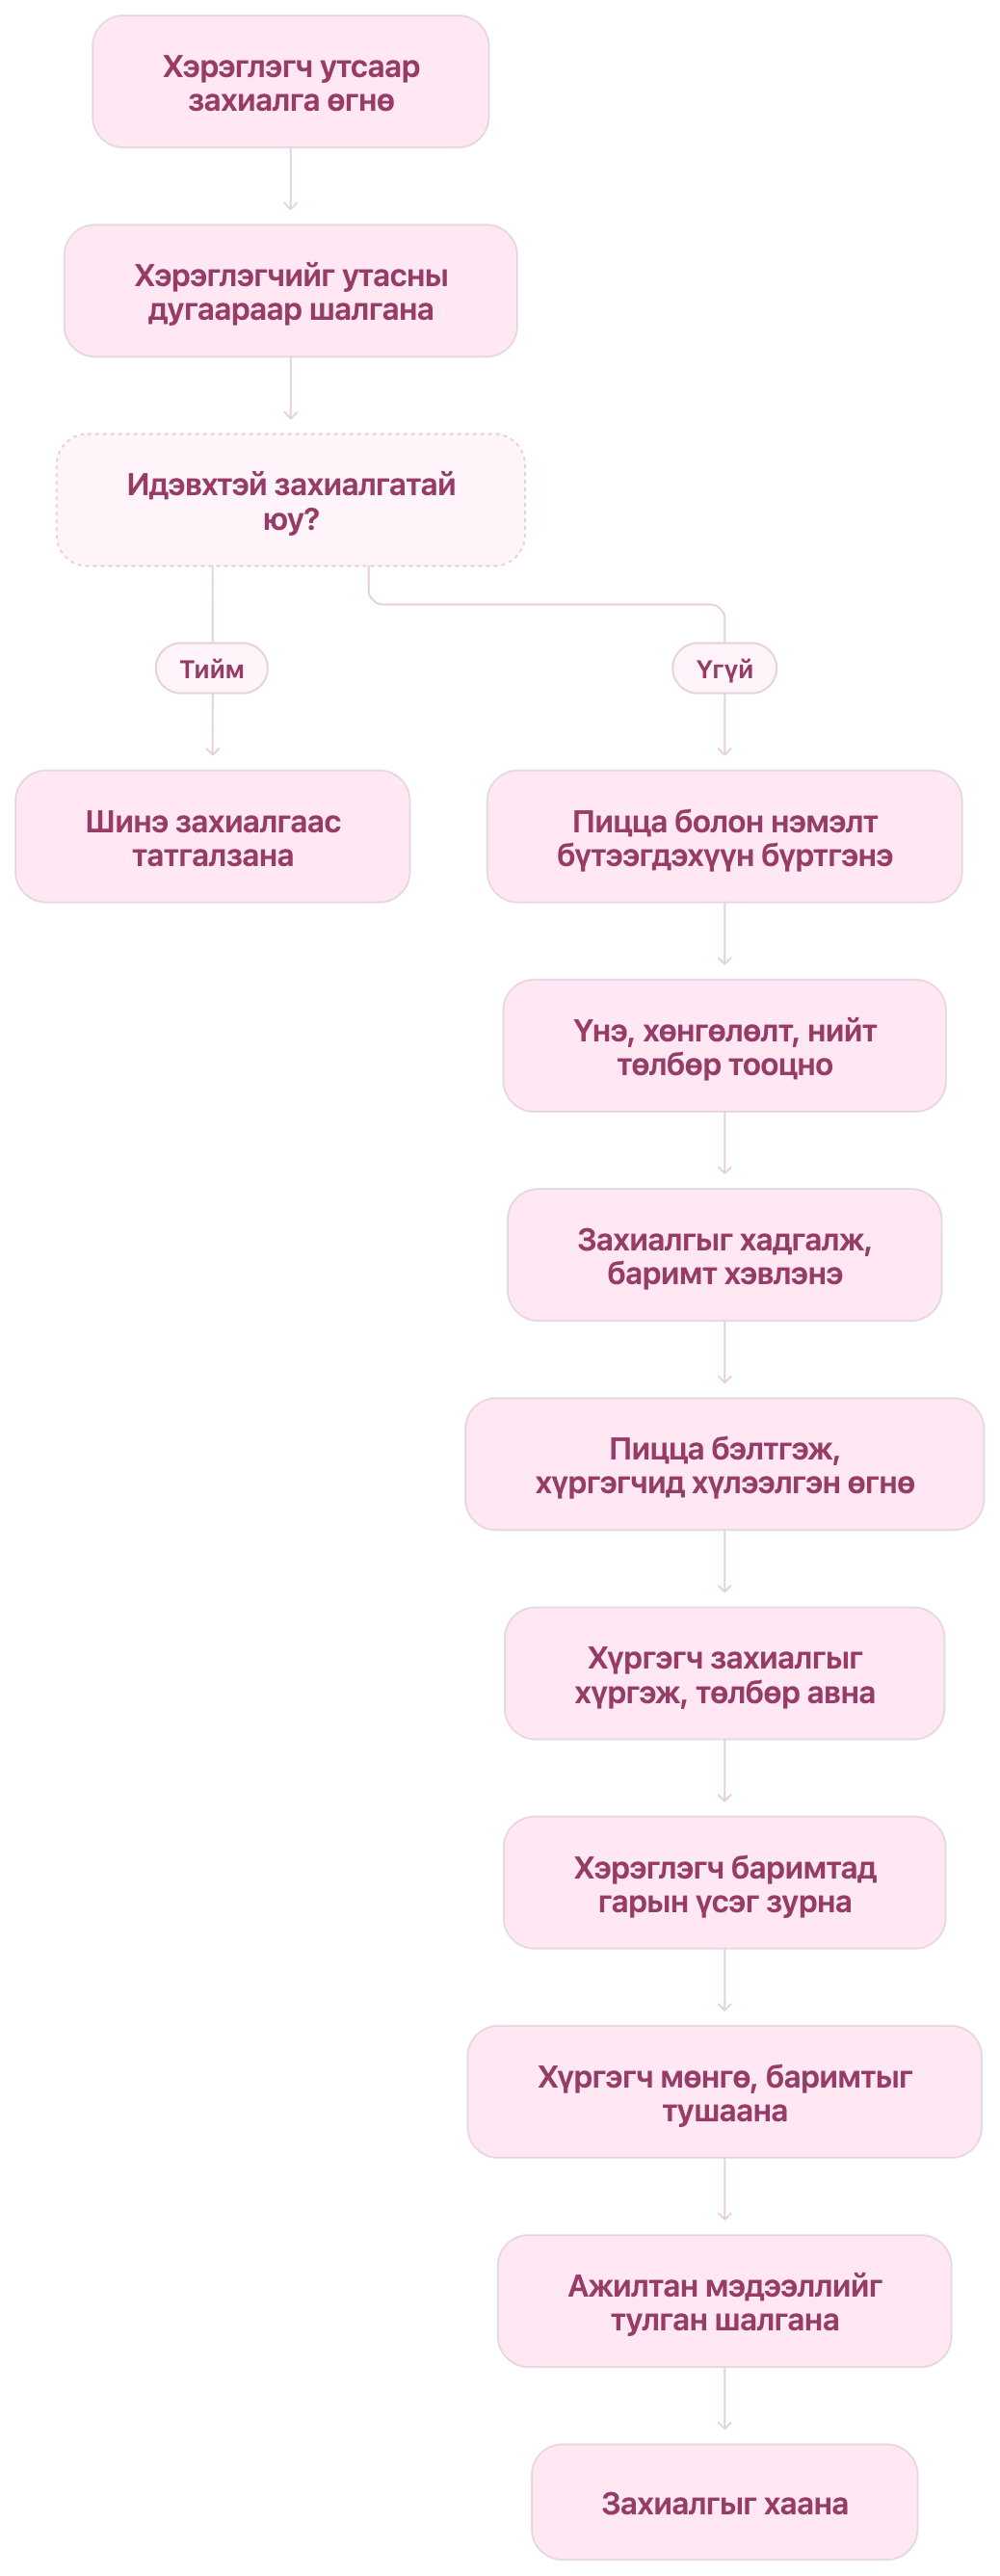
\includegraphics[width=0.65\linewidth]{mermaid-diagram.png}
    \caption{Үндсэн үйл ажиллагааны дараалал}
    \label{fig:placeholder}
\end{figure}


\section{Системийн хамрах хүрээ}
Системийн үндсэн хэрэглэгчид дараах байдлаар байх бөгөөд тэдгээрийн үүргүүдийг дурьдвал

\begin{enumerate}
    \item \textbf{Захиалга хүлээн авагч / бүртгэгч:} 
    Утасны захиалга авах, захиалагчийг шалгах, захиалга бүртгэх, баримт хэвлэх, хүргэгчид захиалга хуваарилах, мөнгө болон гарын үсэгтэй баримтыг хүлээн авч захиалгыг хаах

    \item \textbf{Хүргэгч:} 
    Хүргэлтийн мэдээлэл харах, пицца ба баримт хүлээн авах, захиалгыг хүргэх, төлбөр хураах, хүргэлтийн үр дүнг бүртгэх, мөнгө ба баримтыг тушаах

    \item \textbf{Системийн администратор:} 
    Хэрэглэгчийн бүртгэл болон эрх удирдах, бүтээгдэхүүн, үнэ, хөнгөлөлтийн нөхцөл тохируулах, системийн ажиллагааг хянах

    \item \textbf{Менежер / удирдлага:} 
    Захиалга, борлуулалт, хөнгөлөлт, хүргэлт, төлбөрийн тайлан харах, үйл ажиллагаанд хяналт тавих

\end{enumerate}
Гадаад оролцогчоор Захиалагч байх бөгөөд утсаар захиалга өгч, пицца хүлээн авч, төлбөр төлөн, баримтад гарын үсэг зурна. Гэхдээ системд шууд нэвтрэхгүй тул системийн шууд хэрэглэгч биш, харин бизнес процессын оролцогч юм.

\section{Хэрэглэгчийн шаардлага}

\textbf{1. Захиалга хүлээн авах буюу захиалга бүртгэх функц}
Хэрэглэгч байгууллагын утасны дугаар руу залгаж захиалга өгнө. Захиалга хүлээн авагч системд өөрийн хэрэглэгчийн нэр, нууц үгээр нэвтэрсэн байна.

Захиалга хүлээн авагч хэрэглэгчээс дараах мэдээллийг авна:
\begin{itemize}
    \item нэр;
    \item утасны дугаар;
    \item хүргэлтийн хаяг;
    \item орц, байр, давхар, тоот;
    \item нэмэлт тайлбар;
    \item захиалах бүтээгдэхүүн;
    \item пиццаны төрөл;
    \item пиццаны хэмжээ;
    \item гурилын төрөл;
    \item тоо ширхэг;
    \item нэмэлт орц;
    \item ундаа болон бусад бүтээгдэхүүн;
    \item төлбөрийн хэлбэр.
\end{itemize}

Утасны дугаар нь захиалагчийг таних үндсэн мэдээлэл байна. Системд өмнө нь бүртгэгдсэн хэрэглэгч бол нэр, утас, хүргэлтийн хаягийг автоматаар харуулна. Захиалга хүлээн авагч мэдээллийг шалгаж, шаардлагатай бол шинэчилнэ.

Шинэ хэрэглэгч бол системд хэрэглэгчийн шинэ бүртгэл үүсгэнэ.

\textbf{2. Идэвхтэй захиалгыг шалгах}

Шинэ захиалга үүсгэхээс өмнө систем тухайн утасны дугаартай хэрэглэгчид идэвхтэй захиалга байгаа эсэхийг автоматаар шалгана.

Дараах төлөвтэй захиалгыг идэвхтэйд тооцно:

\begin{itemize}
    \item шинээр бүртгэгдсэн;
    \item баталгаажсан;
    \item бэлтгэгдэж байгаа;
    \item хүргэгчид хуваарилсан;
    \item хүргэлтэд гарсан;
    \item хүргэгдсэн боловч төлбөр тооцоо дуусаагүй;
    \item мөнгө, баримт хүлээгдэж байгаа.
\end{itemize}

Хэрэв хэрэглэгч идэвхтэй захиалгатай бол систем шинэ захиалга хадгалахыг хориглож: \\
“Энэ хэрэглэгчид хаагдаагүй захиалга байна. Өмнөх захиалгыг хаасны дараа шинэ захиалга бүртгэнэ үү.” гэсэн мэдээлэл харуулна.

Хаагдсан болон цуцлагдсан захиалгыг идэвхтэйд тооцохгүй. Ийм хэрэглэгч дахин захиалга өгөх боломжтой.

\textbf{3. Бүтээгдэхүүн сагслах буюу бүтээгдэхүүн сонгох}

Захиалга хүлээн авагч системийн бүтээгдэхүүний жагсаалтаас хэрэглэгчийн сонгосон бүтээгдэхүүнийг сонгоно.

Бүтээгдэхүүн бүр дараах мэдээлэлтэй байна:

\begin{itemize}
    \item бүтээгдэхүүний код;
    \item бүтээгдэхүүний нэр;
    \item ангилал;
    \item хэмжээ;
    \item үндсэн үнэ;
    \item нэмэлт орцын үнэ;
    \item худалдаанд байгаа эсэх;
    \item бэлтгэх боломжтой салбар;
    \item орц, найрлага;
    \item харшил үүсгэж болзошгүй орц.
\end{itemize}

Нэг захиалгад хэд хэдэн төрлийн пицца, ундаа болон нэмэлт бүтээгдэхүүн оруулж болно. Систем бүтээгдэхүүн бүрийн тоо ширхэг болон үнийг үржүүлж мөрийн дүнг автоматаар тооцно.

$$ \text{Мөрийн дүн}=\text{Нэгж үнэ}\times\text{Тоо ширхэг} $$

Бүх бүтээгдэхүүний мөрийн дүнгийн нийлбэрээр захиалгын анхны нийт үнийг олно.

$$ \text{Анхны нийт үнэ}=\sum \text{Бүтээгдэхүүний мөрийн дүн} $$

\textbf{4. Хөнгөлөлт тооцох}

Систем захиалгын анхны нийт үнийг тооцсоны дараа хөнгөлөлтийн нөхцөлийг шалгана.

Бизнесийн үндсэн дүрэм:

\begin{enumerate}
    \item анхны нийт үнэ 40,000 төгрөгөөс дээш бол 20 хувийн хөнгөлөлт олгоно;
    \item анхны нийт үнэ 40,000 төгрөгтэй тэнцүү бол хөнгөлөлт олгохгүй;
    \item анхны нийт үнэ 40,000 төгрөгөөс бага бол хөнгөлөлт олгохгүй.
\end{enumerate}


$$ \text{Хөнгөлөлт}= \begin{cases} \text{Анхны нийт үнэ}\times 0.20, & \text{нийт үнэ}>40,000\\ 0, & \text{нийт үнэ}\leq40,000 \end{cases} $$ $$ \text{Төлөх дүн}=\text{Анхны нийт үнэ}-\text{Хөнгөлөлт} $$

Жишээлбэл, захиалгын анхны нийт үнэ 50,000 төгрөг бол:

$$ 50,000\times20\%=10,000 $$ $$ 50,000-10,000=40,000 $$

Иймд хэрэглэгч 40,000 төгрөг төлнө.

Систем дараах дүнг тусад нь харуулна:

\begin{itemize}
    \item барааны нийт үнэ;
    \item хөнгөлөлтийн хувь;
    \item хөнгөлөлтийн дүн;
    \item хүргэлтийн төлбөр;
    \item төлөх эцсийн дүн.
\end{itemize}

Хүргэлтийн төлбөрийг хөнгөлөлт тооцох анхны үнэд оруулах эсэхийг байгууллагын бизнесийн дүрмээр тусад нь тодорхойлох шаардлагатай.

\textbf{5. Захиалгыг баталгаажуулах}

Мэдээллийг бүрэн оруулсны дараа захиалга хүлээн авагч хэрэглэгчид дараах мэдээллийг дахин уншиж баталгаажуулна:

\begin{itemize}
    \item сонгосон бүтээгдэхүүн;
    \item тоо ширхэг;
    \item нэмэлт орц;
    \item хүргэлтийн хаяг;
    \item анхны үнэ;
    \item хөнгөлөлт;
    \item хүргэлтийн төлбөр;
    \item төлөх эцсийн дүн;
    \item хүргэлтийн ойролцоо хугацаа.
\end{itemize}

Хэрэглэгч зөвшөөрсний дараа ажилтан “Захиалга баталгаажуулах” үйлдлийг сонгоно.

Систем захиалгад давтагдашгүй дугаар үүсгэнэ. Жишээлбэл:

ORD-20260922-00125

Захиалгын анхны төлөв “Бүртгэгдсэн” болно. Систем захиалгыг бүртгэсэн ажилтан, огноо, цагийг автоматаар хадгална.

\textbf{6. Гал тогоонд шилжүүлэх}

Баталгаажсан захиалгыг гал тогоо эсвэл пицца бэлтгэх хэсэгт шилжүүлнэ. Гал тогооны ажилтан дэлгэц эсвэл хэвлэсэн хуудсаас дараах мэдээллийг харна:

\begin{itemize}
    \item захиалгын дугаар;
    \item бүтээгдэхүүний нэр;
    \item хэмжээ;
    \item тоо ширхэг;
    \item нэмэлт болон хасах орц;
    \item хэрэглэгчийн тусгай хүсэлт;
    \item захиалга бүртгэсэн цаг;
    \item бэлэн болгох зорилтот хугацаа.
\end{itemize}

Гал тогоо захиалгыг хүлээн авсны дараа төлөвийг “Бэлтгэгдэж байгаа” болгон өөрчилнө. Пицца бэлэн болсон үед “Бэлэн болсон” төлөвт оруулна.

Бэлтгэх боломжгүй бүтээгдэхүүн илэрвэл захиалга хүлээн авагч хэрэглэгчтэй холбогдож:

\begin{enumerate}
    \item бүтээгдэхүүнийг өөр бүтээгдэхүүнээр солих;
    \item тоо ширхэгийг өөрчлөх;
    \item захиалгын тухайн мөрийг хасах;
    \item захиалгыг бүхэлд нь цуцлах
\end{enumerate}

шийдвэрийн аль нэгийг бүртгэнэ.

\textbf{7. Хүргэгчид захиалга хуваарилах}

Пицца бэлэн болсны дараа захиалга хүлээн авагч эсвэл хүргэлтийн зохицуулагч боломжтой хүргэгчээс сонгоно.

Систем хүргэгч бүрийн дараах мэдээллийг харуулж болно:

\begin{itemize}
    \item хүргэгчийн нэр;
    \item утасны дугаар;
    \item ажиллаж байгаа эсэх;
    \item одоогийн захиалгын тоо;
    \item хүргэлтэд гарсан цаг;
    \item хүргэлтийн бүс;
    \item төлөв.
\end{itemize}

Захиалгыг хүргэгчид хуваарилсны дараа хүргэлтийн баримт хэвлэнэ. Баримтад дараах мэдээлэл байна:

\begin{itemize}
    \item байгууллагын нэр;
    \item захиалгын дугаар;
    \item захиалгын огноо, цаг;
    \item захиалагчийн нэр;
    \item утасны дугаар;
    \item хүргэлтийн хаяг;
    \item бүтээгдэхүүний жагсаалт;
    \item бүтээгдэхүүн бүрийн үнэ;
    \item анхны нийт үнэ;
    \item хөнгөлөлтийн дүн;
    \item хүргэлтийн төлбөр;
    \item төлөх эцсийн дүн;
    \item хүргэгчийн нэр;
    \item хэрэглэгчийн гарын үсэг зурах хэсэг;
    \item хүргэгчийн гарын үсгийн хэсэг;
    \item тусгай тайлбар.
\end{itemize}

Захиалга, пицца болон баримтыг хүргэгч хүлээн авсны дараа системийн төлөвийг “Хүргэлтэд гарсан” болгон өөрчилнө. Хүргэлтэд гарсан огноо, цагийг автоматаар бүртгэнэ.

\textbf{8. Захиалгыг хүргэх}

Хүргэгч баримт болон пиццаг захиалагчийн хаягт хүргэнэ. Хэрэглэгч захиалгаа шалгасны дараа төлбөрийг хүргэгчид өгнө.

Хүргэгч дараах үйлдлийг гүйцэтгэнэ:

\begin{enumerate}
    \item Захиалагчийн нэр, утас, хаягийг тулган шалгах.
    \item Бүтээгдэхүүнийг хэрэглэгчид хүлээлгэн өгөх.
    \item Төлөх эцсийн дүнг баримттай тулгах.
    \item Төлбөрийг бэлэн мөнгөөр хүлээн авах.
    \item Шаардлагатай бол хариулт мөнгө өгөх.
    \item Хэрэглэгчээр хүргэлтийн баримтад гарын үсэг зуруулах.
    \item Хүргэлтийн үр дүнг системд бүртгэх.
\end{enumerate}

Амжилттай хүргэсэн бол захиалгын төлөв “Хүргэгдсэн” болно.

Системд дараах мэдээллийг хадгална:

\begin{itemize}
    \item бодитоор хүлээн авсан мөнгө;
    \item хариулт мөнгө;
    \item хүргэж дууссан цаг;
    \item гарын үсэг авсан эсэх;
    \item хүргэлтийн тайлбар;
    \item хүргэлтийн үр дүн.
    \item 10. Хүргэлт амжилтгүй болох
\end{itemize}

Дараах тохиолдолд хүргэлт амжилтгүй болж болно:

\begin{itemize}
    \item захиалагч утсаа авахгүй байх;
    \item хаяг буруу эсвэл тодорхойгүй байх;
    \item захиалагч заасан хаягт байхгүй байх;
    \item захиалагч захиалга өгөөгүй гэж мэдэгдэх;
    \item захиалагч бүтээгдэхүүнээс татгалзах;
    \item төлбөр хүрэлцэхгүй байх;
    \item хүргэлтийн явцад бүтээгдэхүүн гэмтэх;
    \item цаг агаар, замын нөхцөлөөс шалтгаалан хүргэх боломжгүй болох.
\end{itemize}

Энэ үед хүргэгч “Хүргэлт амжилтгүй” төлөв сонгож, шалтгааныг заавал бүртгэнэ. Захиалга хүлээн авагч хэрэглэгчтэй холбогдон:

\begin{itemize}
    \item дахин хүргэх;
    \item хаягийг засах;
    \item бүтээгдэхүүнийг дахин бэлтгэх;
    \item захиалгыг цуцлах
\end{itemize}

шийдвэр гаргана.

Цуцлагдсан захиалгад цуцалсан ажилтан, шалтгаан, огноо, цагийг хадгална.

\textbf{10. Мөнгө болон баримт тушаах}

Хүргэлт дууссаны дараа хүргэгч байгууллагад буцаж ирэн дараах зүйлсийг захиалга хүлээн авагчид тушаана:

\begin{itemize}
    \item хэрэглэгчээс хүлээн авсан мөнгө;
    \item хэрэглэгчийн гарын үсэгтэй баримт;
    \item амжилтгүй хүргэлтийн бүтээгдэхүүн, хэрэв байгаа бол;
    \item хүргэлтийн нэмэлт тайлбар.
\end{itemize}

Захиалга хүлээн авагч систем дэх төлөх дүнг хүргэгчийн тушаасан мөнгөтэй тулгана.

$$ \text{Зөрүү}=\text{Тушаасан мөнгө}-\text{Системийн төлөх дүн} $$

Зөрүү тэгтэй тэнцүү бол төлбөрийг зөв гэж үзнэ. Зөрүү гарвал систем захиалгыг шууд хаахгүй бөгөөд:

\begin{itemize}
    \item илүү мөнгө;
    \item дутуу мөнгө;
    \item баримт ирээгүй;
    \item гарын үсэг байхгүй;
    \item баримт гэмтсэн
\end{itemize}
гэсэн шалтгааны аль нэгийг бүртгэнэ.

Мөнгө болон баримтыг хүлээн авсны дараа захиалгын төлөвийг “Тооцоо шалгагдаж байгаа” болгоно.

\textbf{11. Захиалгыг хаах}

Захиалгыг хаахаас өмнө систем дараах нөхцөлийг шалгана:

\begin{itemize}
    \item захиалга хүргэгдсэн байх;
    \item төлбөр бүрэн хүлээн авсан байх;
    \item тушаасан мөнгө төлөх дүнтэй тохирсон байх;
    \item гарын үсэгтэй баримт буцаан ирсэн байх;
    \item хүргэгч мөнгө, баримтаа тушаасан байх;
    \item шаардлагатай төлбөрийн баримт үүссэн байх.
\end{itemize}

Бүх нөхцөл хангагдсан бол захиалга хүлээн авагч “Захиалга хаах” үйлдлийг сонгоно. Систем захиалгын төлөвийг “Хаагдсан” болгон өөрчилж, хаасан ажилтан, огноо, цагийг хадгална.

Хаагдсан захиалгыг энгийн хэрэглэгч өөрчлөх боломжгүй. Зөвхөн эрх бүхий администратор үндэслэл бүхий засвар хийж болох бөгөөд бүх өөрчлөлтийг аудитын бүртгэлд хадгална.

Захиалга хаагдсаны дараа тухайн хэрэглэгч шинэ захиалга өгөх боломжтой болно.

\section{Функциональ шаардлага}

\textbf{Захиалга хүлээн авагчийн функциональ шаардлага}
\begin{enumerate}
    \item захиалагчийг хайх, бүртгэх;
    \item идэвхтэй захиалга шалгах;
    \item захиалга үүсгэх, засах;
    \item бүтээгдэхүүн сонгох;
    \item хөнгөлөлт шалгах;
    \item хүргэгч хуваарилах;
    \item баримт хэвлэх;
    \item мөнгө, баримт хүлээн авах;
    \item захиалга хаах.
\end{enumerate}

\textbf{Хүргэгчийн функциональ шаардлага}
\begin{itemize}
    \item өөрт хуваарилсан захиалгыг харах;
    \item пицца болон баримт хүлээн авах;
    \item хүргэлтэд гарсныг бүртгэх;
    \item хүргэлтийн үр дүн оруулах;
    \item төлбөрийн дүн бүртгэх;
    \item мөнгө, баримт тушаах.
\end{itemize}

\textbf{Менежерийн функциональ шаардлага}
\begin{itemize}
    \item бүх захиалга харах;
    \item хөнгөлөлтийн дүрэм тохируулах;
    \item хүргэлтийн ажиллагааг хянах;
    \item мөнгөний зөрүү шалгах;
    \item борлуулалтын тайлан харах;
    \item цуцлалт болон буцаалтыг батлах.
\end{itemize}
    
\textbf{Системийн администраторын функциональ шаардлага}
\begin{itemize}
    \item хэрэглэгчийн бүртгэл үүсгэх;
    \item хэрэглэгчийн эрх тохируулах;
    \item бүтээгдэхүүн, үнэ удирдах;
    \item системийн тохиргоо хийх;
    \item аудитын бүртгэл харах;
    \item мэдээллийн нөөцлөлт, хамгаалалтыг удирдах.
\end{itemize}

\textbf{Тайлангийн үйл ажиллагаа}

Систем дараах тайланг гаргах боломжтой байна:
\begin{itemize}
    \item өдөр, долоо хоног, сарын борлуулалт;
    \item нийт захиалгын тоо;
    \item хаагдсан болон цуцлагдсан захиалга;
    \item хөнгөлөлттэй захиалгын тоо, дүн;
    \item хамгийн их борлуулалттай бүтээгдэхүүн;
    \item хүргэгч бүрийн хүргэлтийн тоо;
    \item хүргэлтийн дундаж хугацаа;
    \item амжилтгүй хүргэлтийн шалтгаан;
    \item бэлэн мөнгөний орлого;
    \item мөнгөний илүү, дутуу зөрүү;
    \item хэрэглэгчийн гомдол;
    \item давтан захиалгын мэдээлэл.
\end{itemize}

\subsection{Системийн үндсэн бизнес дүрэм}
\begin{itemize}
    \item Нэг хэрэглэгч нэгэн зэрэг нэг л идэвхтэй захиалгатай байна.
    \item 40,000 төгрөгөөс дээш захиалгад 20 хувийн хөнгөлөлт олгоно.
    \item Хөнгөлөлтийг систем автоматаар тооцно.
    \item Хөнгөлөлтийг энгийн ажилтан гараар өөрчлөх боломжгүй байна.
    \item Захиалга бүр давтагдашгүй дугаартай байна.
    \item Хүргэгч зөвхөн өөрт хуваарилсан захиалгыг харна.
    \item Хүргэлтэд гарсан захиалгын бүтээгдэхүүн, үнийг зөвшөөрөлгүй өөрчлөхгүй.
    \item Мөнгө болон гарын үсэгтэй баримт ирээгүй бол захиалгыг хаахгүй.
    \item Төлбөрийн дүн зөрүүтэй бол захиалгыг хаахгүй.
    \item Зөвхөн эрх бүхий ажилтан захиалгыг цуцлах болон хаах боломжтой.
    \item Захиалгын төлөвийн өөрчлөлт бүрийг аудитын бүртгэлд хадгална.
    \item Хаагдсан захиалгыг зассан бүх тохиолдолд шалтгаан заавал бичнэ.
\end{itemize}

Ингэснээр систем нь захиалга бүртгэх энгийн программаас илүүтэйгээр захиалагч, захиалга хүлээн авагч, гал тогоо, хүргэгч, төлбөр тооцоо болон удирдлагыг нэг урсгалд холбосон нэгдсэн мэдээллийн систем болно

\section{Функционал бус шаардлага}

\subsection{Гүйцэтгэлийн шаардлага}
\begin{itemize}
    \item Хэрэглэгчдэд ойлгомжтой, энгийн интерфэйстэй байх.
    \item Дэлгэц шилжих хурд хамгийн ихдээ 10 секунд байх.
    \item Өвчтөний мэдээлэл болон эмийн мэдээлэл харах хурд 3-10 секунд байх.
    \item Өгөгдлийн сангийн ачаалал хурдан шуурхай байх.
\end{itemize}

\subsection{Аюулгүй байдлын шаардлага}
\begin{itemize}
    \item Сервер, өгөгдлийн сангийн аюулгүй байдлыг хангах.
    \item Өвчтөн, ажилтны мэдээлэл алдагдахгүй байх.
    \item Системийн нэвтрэлт зөвшөөрөгдсөн хэрэглэгчдэд зориулагдсан байх.
\end{itemize}

\subsection{Хамгаалалт, нууцлалын шаардлага}
\begin{itemize}
    \item Эмч, эмийн санч, хэрэглэгчийн мэдээллийг нууцлалтай хадгалах.
    \item Нууц үг дэлгэцэнд харуулахгүй байх.
    \item Сервер болон өгөгдлийн санг нууц хамгаалалттай байлгах.
\end{itemize}

\subsection{Программ хангамжийн чанарын шаардлага}
\begin{itemize}
    \item Ашиглахад хялбар, ойлгомжтой байх.
    \item Шинэчлэл хийх боломжтой байх.
    \item Монгол хэл дээр ажиллах.
    \item Систем нэгэн зэрэг олон хэрэглэгчийн хандалтыг дэмжих.
\end{itemize}

\section{Ашигласан технологи, техникийн шаардлага}

\subsection{Технологийн шаардлага}

\subsubsection{Программ ажиллах үйлдлийн системийн сонголт}
\qquad
Энэхүү эмийн систем нь мобайл болон вэб орчинд ажиллана. Мобайл үйл ажиллагааг дэмждэг бүх төхөөрөмж дээр веб браузерээр ажиллах боломжтой. Программ хангамжийн дэмжих үйлдлийн системүүд:

\begin{enumerate}
    \item Android үйлдлийн систем
    \item iOS үйлдлийн систем
    \item Windows үйлдлийн систем
    \item macOS үйлдлийн систем (заавал шаардлагатай бол)
\end{enumerate}

\subsubsection{Өгөгдлийн сангийн удирдах системийн сонголт}
\qquad
Энэхүү системийн өгөгдлийн сангийн баазыг MongoDB өгөгдлийн сан удирдах систем дээр хөгжүүлэхээр төлөвлөсөн. MongoDB нь NoSQL төрлийн өгөгдлийн сан бөгөөд дараах давуу талуудтай:

\begin{itemize}
    \item Их хэмжээний өгөгдлийг хурдан боловсруулж хадгалах
    \item Өвөрмөц бүтэцтэй өгөгдлийг хялбар удирдах
    \item Өндөр аюулгүй байдал, нөөцлөлт, сэргээх боломжтой
    \item Програмын хөгжүүлэлтэд уян хатан байдлыг хангах
\end{itemize}

\subsection{Техникийн шаардлага}
\subsubsection{Оролт гаралтын төхөөрөмжүүдийн шаардлага}

\begin{longtable}{| p{0.7cm} | p{4cm} | p{3.5cm} | p{3.3cm} |}
		\hline
		\textbf{№} & \textbf{Төхөөрөмж} & \textbf{Төрөл} & \textbf{Шаардлага}\\
		\hline
		1 & \begin{center}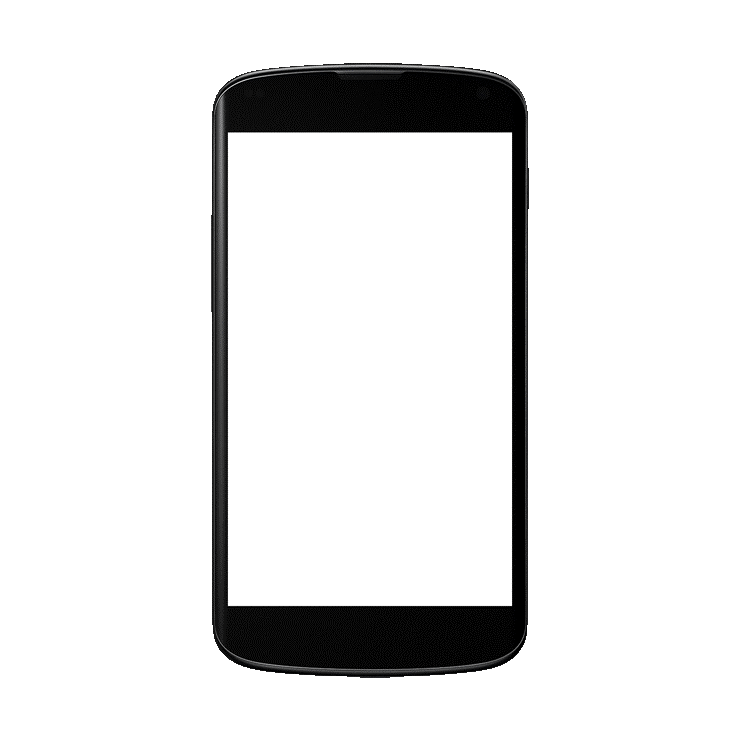
\includegraphics[width=2cm]{Figures/icon1} \end{center}& Мэдрэх & Энгийн  \\
		\hline
		2 & \begin{center}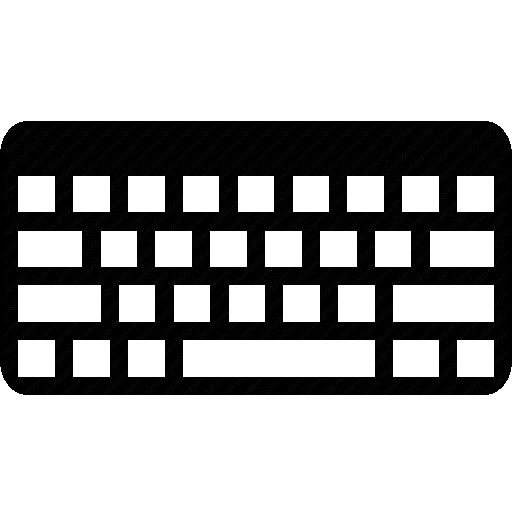
\includegraphics[width=2cm]{Figures/icon2} \end{center} & Оролт & Энгийн \\
		\hline
		3 & \begin{center}
\includegraphics[width=2cm]{Figures/icon3} \end{center} & Гаралт & Дурын  \\
		\hline
		4 & \begin{center}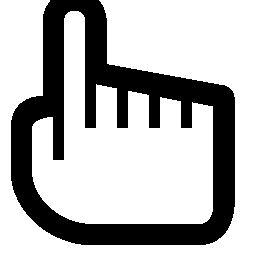
\includegraphics[width=2cm]{Figures/icon4} \end{center} & Заах & Дурын \\
		\hline
		\caption[Оролт гаралтын төхөөрөмжүүдийн шаардлага]{Оролт гаралтын төхөөрөмжүүдийн шаардлага}

	\end{longtable}


    

\section{Юзкейс диаграм}

.... 

%-------------------------------------------------------------------------------
%	THESIS CONTENT - APPENDICES
%-------------------------------------------------------------------------------

\appendix % Дараах "chapters" нь Хавсралт болохыг LaTex -д хэлэх

\include{Appendices/AppendixA}

%-------------------------------------------------------------------------------
%	BIBLIOGRAPHY
%-------------------------------------------------------------------------------
\defformat % Бүлгийн нэрийг оргиналь байдлаар хэвлэх

\addchaptertocentry{Ном зүй} % Ном зүйг гарчигт нэмэх

\printbibliography[heading=bibliography,title={Ном зүй}]

%-------------------------------------------------------------------------------
\end{document}